\documentclass[12pt,a4paper]{article}
\PassOptionsToPackage{hidelinks}{hyperref}
% Preambule commun aux comptes rendus CR_*.tex.

\usepackage{array}
\newcolumntype{C}[1]{>{\centering\arraybackslash}m{#1}}
\usepackage{multirow}
\usepackage{geometry}
\geometry{a4paper, margin=1in}
\usepackage{graphicx}
\usepackage{float}
\usepackage{tikz}
\usetikzlibrary{arrows.meta,positioning}
\usepackage{pgfgantt}
\usepackage{pdflscape}
\usepackage{enumitem}
\usepackage{booktabs}
\usepackage{longtable}
\usepackage{ragged2e}
\usepackage{tabularx}
\usepackage{xparse}
\usepackage{ltablex}
\usepackage{xltabular}
\usepackage{subcaption}

\newcolumntype{Y}{>{\RaggedRight\arraybackslash}X}

\newcommand{\StyledTableSetup}{%
  \footnotesize
  \renewcommand{\arraystretch}{1.2}%
  \setlength{\tabcolsep}{4pt}%
}


% ============================================================
% IHEDN COVER TEMPLATE (XeLaTeX)
% ============================================================
% Compilation (from project root):
%   latexmk -pdf main.tex
%   LATEXMK_SHELL_ESCAPE=0 latexmk -pdf main.tex
%
% Optional environment controls from latexmkrc:
%   LATEXMK_ENGINE=xelatex        (default/enforced)
%   LATEXMK_SHELL_ESCAPE=1|0      (default 1, needed for SVG conversion)
%
% Required package for this template:
%   \usepackage{ihedn-cover}
%
% Note: ihedn-cover already loads needed internal packages
% (fontspec, graphicx, tikz, ragged2e, optional svg).
% ============================================================

% ----------------------------------------------------------------
% Package options (documented)
% ----------------------------------------------------------------
% Geometry scope:
%   apply-geometry            -> force A4 + zero margins while cover is built
%   no-apply-geometry         -> do not alter host geometry (default)
%
% Typesetting freeze:
%   global-typesetting        -> apply freeze globally (intrusive)
%   no-global-typesetting     -> no global freeze (default)
%
% Small-caps handling:
%   local-smallcaps-fix       -> \textsc -> \MakeUppercase only inside cover (default)
%   no-local-smallcaps-fix    -> disable local fix
%   global-smallcaps-fix      -> global override (intrusive)
%   no-global-smallcaps-fix   -> disable global fix (default)
%
% Main font handling:
%   global-mainfont           -> set Times New Roman globally (default)
%   local-mainfont            -> set Times only during cover rendering
%   no-mainfont-override      -> keep host document main font
%
% SVG support:
%   svg-support               -> enable SVG logos (default, needs shell-escape)
%   no-svg-support            -> disable SVG path handling (pdf/png only)
%
% Debug overlay:
%   debug                     -> show mm grid + bounding boxes on cover
%   no-debug                  -> hide debug overlay (default)
% ----------------------------------------------------------------
\usepackage[
  no-apply-geometry,
  no-global-typesetting,
  global-smallcaps-fix,
  local-smallcaps-fix,
  global-mainfont,
  svg-support,
  no-debug
]{ihedn-cover}

% ----------------------------------------------------------------
% Bibliography stack (BibLaTeX/Biber, style from subtree vendor/)
% ----------------------------------------------------------------
\usepackage{polyglossia}
\setdefaultlanguage{french}
\makeatletter
\g@addto@macro\captionsfrench{%
  \renewcommand{\tablename}{Tableau}%
  \renewcommand{\figurename}{Figure}%
}
\makeatother
\usepackage{csquotes}
\usepackage{xurl}
\usepackage{hyperref}
\makeatletter
\let\ihedn@orig@input@path\input@path
\def\input@path{{vendor/biblatex-sciences-po-fr/style/}}
\makeatother
\usepackage[
  backend=biber,
  style=sciencespo,
  hyperref=true,
  autolang=other
]{biblatex}
\AtBeginBibliography{\sloppy\setlength{\emergencystretch}{3em}}
\makeatletter
\let\input@path\ihedn@orig@input@path
\makeatother
\addbibresource{bibliographies/bib/rapport.bib}

% ----------------------------------------------------------------
% tcolorbox
% ----------------------------------------------------------------
\usepackage[most]{tcolorbox}
\tcbuselibrary{breakable}

% Example: use Arial for the full report + cover.
% Uncomment and switch package option to no-mainfont-override.
% \setmainfont{Arial}[
%   UprightFont    = *,
%   BoldFont       = * Bold,
%   ItalicFont     = * Italic,
%   BoldItalicFont = * Bold Italic
% ]

%==================================================
% Liste des propositions
%==================================================

\makeatletter

\newcommand{\listpropositionname}{Liste des propositions}

\newcommand{\listofpropositions}{
  \section*{\listpropositionname}
  \addcontentsline{toc}{section}{\listpropositionname}
  \@starttoc{lop}
}

\newcommand*\l@proposition{\@dottedtocline{1}{1.5em}{2.3em}}

\makeatother

%==================================================
% Compteur des propositions
%==================================================

\newcounter{proposition}

%==================================================
% Style graphique des propositions
%==================================================

\newtcolorbox{propositionbox}[2][]{
  lower separated=false,
  colback=white!80!gray,
  colframe=white!20!black,
  fonttitle=\bfseries,
  colbacktitle=white!30!gray,
  coltitle=black,
  enhanced,
  sharp corners,
  attach boxed title to top left={
    xshift=0.5cm,
    yshift=-2mm
  },
  title=#2,
  #1
}

%==================================================
% Environnement proposition
%==================================================

\newenvironment{proposition}[1]
{
  \refstepcounter{proposition}

  \addcontentsline{lop}{proposition}{%
    \protect\numberline{\theproposition}#1%
  }

  \begin{propositionbox}
  {Proposition~\theproposition~: #1}
}
{
  \end{propositionbox}
}

% Renommage Liste des figures en Table des figures
\addto\captionsfrench{%
  \renewcommand{\listfigurename}{Table des figures}
}

\newcommand{\heure}[2]{{\NoAutoSpacing #1:#2}}

\DeclareFieldFormat[misc]{title}{#1}

% Activer ce package avec l'option none retire la césure.
%\usepackage[none]{hyphenat}

\usepackage{adjustbox}
\usepackage{pdfpages}

\makeatletter
\newcommand{\IhednSetPdfPageCount}[2]{%
  \begingroup
  \edef\ihedn@pdfpath{#2}%
  \ifXeTeX
    \global#1=\XeTeXpdfpagecount "\ihedn@pdfpath" %
  \else
    \ifLuaTeX
      \saveimageresource{\ihedn@pdfpath}%
      \global#1=\lastsavedimageresourcepages\relax
    \else
      \pdfximage{\ihedn@pdfpath}%
      \global#1=\pdflastximagepages\relax
    \fi
  \fi
  \endgroup
}
\makeatother

\newcount\IhednIncludedPdfPageCount
\newcommand{\IhednRenderPdfPagesInBoxes}[1]{%
  \IhednSetPdfPageCount{\IhednIncludedPdfPageCount}{#1}%
  \foreach \IhednIncludedPdfPage in {1,...,\the\IhednIncludedPdfPageCount}{%
    \begin{tcolorbox}[
      colback=gray!5,
      colframe=black,
      boxrule=0.5pt,
      arc=3mm
    ]
    \centering
    \includegraphics[page=\IhednIncludedPdfPage,width=0.95\textwidth]{#1}
    \end{tcolorbox}
    \ifnum\IhednIncludedPdfPage<\IhednIncludedPdfPageCount
      \clearpage
    \fi
  }%
}

\usepackage{tablefootnote}


\usepackage[acronym,toc,section=section]{glossaries}
\makeglossaries
% ---------- Acronymes ----------
\newacronym{codir}{CODIR}{Comité de direction}
\newacronym{dreal}{DREAL}{Direction régionale de l'environnement, de l'aménagement et du logement}
\newacronym{dmd}{DMD}{Délégué Militaire Départemental}
\newacronym{retex}{RETEX}{Retour d'expérience}
\newacronym{orsec}{ORSEC}{Organisation de la Réponse de SEcurité Civile}
\newacronym{pcis}{PCIS}{Plans intercommunaux de sauvegarde}
\newacronym{pcs}{PCS}{Plan communal de sauvegarde}
\newacronym{rgpd}{RGPD}{Règlement général sur la protection des données}
\newacronym{irsem}{IRSEM}{Institut de recherche stratégique de l'École militaire}
\renewcommand*{\acronymname}{Liste des acronymes}

\begin{document}

% ----------------------------------------------------------------
% Cover keys (all available keys are shown below)
% ----------------------------------------------------------------
% Header block (top-right), logo, title, report lines, subtitle, committee.
\PageDeGardeIHEDN{
    header_1={Union-IHEDN},
    header_2={Association des auditeurs IHEDN},
    header_3={région Paris / Île de France},
    date={le \today},
    logo_path={Figures/logos_IHEDN/Logo_AR_16_PARIS_IDF.jpg},
    title={Crises majeures : quel rôle pour les citoyens engagés et les associations IHEDN ?},
    title_max_lines=2,
    title_fontsize={26.000pt},
    title_baselineskip={28.667pt},
    reportline_1={Rapport du Comité d'étude de l'Association régionale des auditeurs},
    reportline_2={de l'IHEDN région Paris / Île de France (AR 16)},
    subtitle={},
    committee={Comité d'étude, d'octobre 2025 à juin 2026, composé de : Mme Valérie Arlé-Faivre, \textit{présidente} ; M. Aurélien Duvignac-Rosa, \textit{rapporteur} ; M. Pascal Bayot Duponchel ; M. Jean-Jacques Cleynen ; Mme Valérie Cowan ; M. Alain Fontan ; M. Pierre-Marie Giard ; Mme Muriel Joyeux ; M. Bruno Leray ; M. Yves-Henri Renhas ; M. Marc Roure ; Mme Isabelle de Segonzac ; M. Gérard Turck ; Mme Marie Danielle Vasquez-Duchêne.}
}

% --- Pages liminaires en chiffres romains ---
\pagenumbering{Roman}

\addcontentsline{toc}{section}{Résumé}
\section*{Résumé}

Face à l'émergence de crises de plus en plus complexes et systémiques : climatiques, sécuritaires, technologiques ou informationnelles, les associations de l'IHEDN sont appelées à apporter une contribution tangible et structurée. Dans ce contexte, leur valeur ajoutée se situe principalement en amont et en aval des crises, à travers des actions de préparation, de sensibilisation, d'analyse et de retour d'expérience.

Toutefois, la mobilisation effective de ces compétences suppose préalablement une connaissance fine et objectivée des profils, d'un point de vue expertise et capacitaire d'engagement des membres. Dans cette perspective, la mise en place d'un questionnaire visant à cartographier les compétences au sein des différentes associations apparaît comme une objectif pertinent et justifié.

Une telle démarche, pour être pleinement opérante, doit néanmoins s'inscrire dans un cadre méthodologique rigoureux et s'appuyer sur un plan prévisionnel précis, condition indispensable pour garantir la fiabilité des données recueillies, la pertinence des analyses produites et, \textit{in fine}, la crédibilité du dispositif proposé.

Le présent rapport vise à présenter de manière structurée l'ensemble des éléments susmentionnés.

\clearpage

\tableofcontents

\clearpage
\addcontentsline{toc}{section}{Table des figures}

\listoffigures

\clearpage

% --- Corps du document en chiffres arabes ---
\pagenumbering{arabic}

\section{Introduction}

Les crises majeures auxquelles les pouvoirs publics sont désormais confrontés prennent des formes plus diverses et plus imbriquées : sanitaires, environnementales, technologiques, sécuritaires\footcite{AN:2022:Resilience_nationale} ou encore informationnelles\footcite[3]{SciencesPo:2025:Resilience_menaces_informationnelles}. Elles interrogent directement la capacité de la société à se préparer, à absorber les chocs et à en tirer les enseignements durables.

Cette évolution se manifeste notamment par le développement des formes de conflictualité dites « hybrides\footcite{tenenbaum2016guerre} » et dans l'amplification des phénomènes de désinformation par les réseaux sociaux\footcite{garrigou2025desinformation}. Les frontières traditionnelles entre temps de paix, temps de crise et confrontation ouverte s'en trouvent moins nettes, ce qui rend plus difficile la seule réponse par des dispositifs institutionnels spécialisés.

La planification et la mise en place de solutions de gestion de crise ne peuvent donc plus être envisagées uniquement sous l'angle des autorités compétentes. Elles supposent également une meilleure articulation avec les compétences disponibles au sein de la société civile organisée, en particulier lorsqu'elles peuvent être identifiées, qualifiées et mobilisables dans un cadre clair\footcite{AN:2022:Resilience_nationale}.

Cette préoccupation rejoint les évolutions récentes du cadre européen de défense. La Commission européenne a ainsi dévoilé, le 19 mars 2025\footcite{burgdorff2025livreblanc}, dans un contexte marqué par la menace russe, un livre blanc pour la défense européenne destiné à définir le périmètre du plan ReArm Europe à l'horizon 2030\footcite{viepublique2025livreblanc}. Au-delà de sa dimension capacitaire, cette dynamique souligne que la préparation aux crises engage aussi la cohésion, l'information et la mobilisation des sociétés.

Dans ce prolongement, les initiatives récentes engagées au niveau national traduisent également une volonté de mieux associer la société à la préparation des crises. Le projet de service national, tel que présenté par le gouvernement français en 2026, s'inscrit dans cette dynamique en visant à impliquer davantage les jeunes générations dans des missions utiles à la défense nationale.

Les appelés du service national sont ainsi appelés à développer des savoir-faire reconnus au travers de missions relevant de trois grands domaines : la protection du territoire, le soutien au fonctionnement quotidien des armées et l'apport d'expertises dans des domaines techniques ou spécialisés\footcite{info_gouv_service_national}.

Toutefois, ce dispositif ne s'inscrit pas dans une logique de retour à une conscription généralisée, comme l'a rappelé le général Pierre Schill, chef d'état-major de l'armée de Terre\footcite{leparisien_schill_service_national}. Il traduit plutôt une évolution des modalités d'engagement, fondée sur une participation ciblée et adaptée aux besoins contemporains.

C'est dans ce cadre que les échanges relatifs aux travaux du comité se sont appuyés sur l'hypothèse de travail suivante : les associations de l'IHEDN, et en particulier l'Association régionale Paris Île-de-France (AR 16), peuvent contribuer utilement à cette réflexion, à condition de préciser la nature réelle de cet apport, ses limites et ses modalités possibles. Le présent rapport de comité s'attache ainsi à examiner la problématique suivante :

\begin{quote}
\textbf{Crises majeures : quel rôle pour les citoyens engagés et les associations IHEDN ?}
\end{quote}

L'objectif de ce travail est d'analyser la capacité de contribution des auditeurs IHEDN à la gestion des crises majeures, d'identifier leur plus-value spécifique et de distinguer les formes d'engagement les plus pertinentes, notamment en amont de la crise et dans les démarches de retour d'expérience. Cette analyse conduit également à poser la question d'une connaissance plus précise des profils, des compétences et des disponibilités des membres, condition nécessaire à toute mobilisation structurée.

\clearpage

\section{Cadre général et enjeux contemporains}

\subsection{Une approche en termes de sécurité globale}

Les crises majeures relèvent désormais d'un registre d'action multidimensionnel : militaire, civil, économique ou encore sociétal.

Ce cadre d'analyse évite de limiter la réflexion aux seuls dispositifs publics de gestion de crise, même si ceux-ci en constituent naturellement le socle. Il conduit à prendre en compte les compétences présentes dans des réseaux associatifs, professionnels et citoyens, dès lors que leur contribution peut être identifiée et organisée. À ce titre, l'Association régionale Île-de-France de l'IHEDN (AR~16) constitue un terrain d'observation très intéressant : elle rassemble des membres issus d'administrations, des forces armées, d'entreprises, du monde académique et de la société civile, avec des expériences et des savoir-faire complémentaires.

\subsection{L'évolution des menaces : vers des crises systémiques}

Les travaux du comité ont d'abord conduit à identifier plusieurs familles de menaces susceptibles de provoquer ou d'aggraver des crises majeures : l'intensification des risques climatiques et énergétiques\footcite{AN:2022:Resilience_nationale}, la montée en puissance des cybermenaces\footcite{Berthier_hacktivisme}, ainsi que le développement des stratégies d'affrontement hybride\footcite{Gere_affrontement_hybride}.

Ces stratégies hybrides peuvent être analysées à travers trois modalités. La première est la dissuasion : elle vise à maintenir un rapport de force et de tension entre nations, sans franchir le seuil du conflit ouvert\footcite[p.89]{Gere_affrontement_hybride}. La deuxième est la dissimulation, qui repose sur le recours à des acteurs indirects, tels que des mercenaires ou des groupes para-étatiques, ainsi que sur des actions clandestines comme les cyberattaques, afin de brouiller l'attribution des responsabilités\footcite[p.90]{Gere_affrontement_hybride}. La troisième concerne la désinformation, qui utilise les vecteurs de diffusion de l'information pour amplifier les succès du camp émetteur, minimiser ses échecs et fragiliser la perception et la cohésion du pays cible\footcite[p.91]{Gere_affrontement_hybride}.

Ce dernier point est renforcé par les réseaux sociaux qui accélèrent la circulation de récits hostiles, fragilisent la confiance envers les institutions et contribuent à amplifier les effets d'une crise déjà engagée\footcite{Sibony_reseaux_sociaux_et_guerre}.

Dans ce contexte, le comité a retenu une approche prudente du positionnement de l'AR~16 : non comme un acteur direct de la gestion de crise, mais comme un réseau dont les compétences doivent être mieux connues afin d'en apprécier la contribution réelle.

\clearpage

\section{Problématique et positionnement de l'AR 16}

\subsection{Une contribution indirecte mais stratégique}

Les travaux du comité conduisent à poser le cadre de départ suivant :

\begin{quote}
\textbf{L'AR 16 n'a pas vocation à gérer directement les crises, mais à contribuer à leur préparation, à leur accompagnement et à leur analyse.}
\end{quote}

Ce positionnement conduit à se situer en complément des dispositifs existants, sans chercher à s'y substituer. L'apport possible de l'association doit donc être envisagé au regard des missions exercées par les autorités publiques, en identifiant les domaines où les compétences des auditeurs peuvent utilement renforcer la préparation, l'appui ou l'analyse.

\subsection{Identification de la valeur ajoutée des auditeurs}

Dans un environnement de gestion de crise déjà structuré (\gls{orsec}\footcite{ORSEC_def}, \gls{pcs}, \gls{pcis}\footcite{PCS_PICS_def}, sécurité civile), la question n'est pas de créer un rôle supplémentaire. Elle consiste d'abord à déterminer ce que les membres de l'AR~16 peuvent apporter concrètement, puis à situer cet apport dans les phases du cycle de crise où il est le plus pertinent.

Cette clarification permet d'éviter une mobilisation trop générale, difficilement exploitable par les acteurs publics, tout en distinguant les contributions qui relèvent de l'expérience professionnelle des auditeurs de celles qui peuvent être portées collectivement par le réseau associatif.

Les réflexions convergent vers la réponse suivante : \textbf{cet apport se situe principalement en amont et en aval des crises}.

\clearpage

\section{Temporalité de l'engagement des auditeurs}

Pour apprécier la contribution possible des auditeurs, le comité a choisi de raisonner selon les trois phases du cycle de crise. Cette approche permet de distinguer ce qui relève de la préparation, ce qui peut être envisagé pendant l'événement, et ce qui prend sens dans l'analyse \textit{a posteriori}.

\subsection{Avant la crise : préparation et résilience}

En amont, les auditeurs contribuent à diffuser une culture de sécurité, à sensibiliser les populations et à participer à des dispositifs de préparation, notamment autour des \gls{pcs}\footcite{PCS_PICS_def} ou d'exercices à destination des populations\footcite{Gestion_de_crise_def_exemples}.

\subsection{Pendant la crise : une place limitée}

Lorsque la crise est engagée, le cadre d'action se resserre rapidement. La gestion de crise obéit à une organisation strictement hiérarchisée, au sein de laquelle les auditeurs interviennent principalement au titre de leurs fonctions professionnelles.

Dans ce contexte, la contribution directe de l'association en tant que telle demeure limitée, l'expérience de ses membres s'exerçant principalement dans le cadre de leurs responsabilités propres.

\subsection{Après la crise : analyse et \acrshort{retex}}

En aval, la valeur ajoutée des auditeurs se précise. Leur expérience et la diversité de leurs parcours peuvent nourrir l'analyse des crises, la participation aux retours d'expérience (\acrshort{retex}) et l'élaboration de recommandations.

Cette lecture temporelle confirme que l'enjeu n'est pas seulement de définir une intention générale de mobilisation. Il s'agit d'abord de mieux connaître les profils, les compétences et les disponibilités des membres de l'AR~16, afin d'identifier les contributions possibles et les conditions dans lesquelles elles pourraient s'organiser.

\clearpage

\section{Proposition structurante : le questionnaire}

\subsection{Un enjeu central : mieux connaître et mobiliser les auditeurs}

Les travaux du comité ont fait émerger un constat clair :

\begin{quote}
\textbf{Le potentiel des auditeurs IHEDN est important mais insuffisamment identifié et structuré.}
\end{quote}

L'annuaire existant reste lacunaire. Il ne permet pas, en l'état, d'identifier avec suffisamment de précision les compétences susceptibles d'être mobilisées.

Cette limite ne permet pas de valoriser pleinement les capacités de l'association. La mise en place d'un outil dédié apparaît donc comme une étape préalable pour mieux connaître les profils, apprécier les disponibilités et préparer, le cas échéant, une mobilisation adaptée.

\subsection{Une démarche d'objectivation}

Le comité propose de recourir à un questionnaire afin de disposer d'une connaissance plus fiable et plus exploitable des membres.

Cette démarche pourrait s'inscrire dans le cadre du cinquantième anniversaire de l'association\footcite{linkedin_AR16}. Cette échéance offre un cadre pertinent pour engager une réflexion collective sur l'histoire de l'association et sur sa capacité d'adaptation face aux défis contemporains.

Le questionnaire visa à recueillir des données qualitatives et quantitatives utiles pour apprécier les formes possibles d'implication des membres des associations de l'IHEDN. Cette réflexion s'inscrit dans la continuité de travaux antérieurs, notamment ceux relatifs à la création d'une réserve de l'IHEDN, étudiée à la demande d'Édouard Philippe en 2015\footcite{DESAINTSALVY2026}.

Elle trouve également un écho dans des analyses récentes émanant de personnalités de premier plan au sein de l'IHEDN. Ainsi, comme le souligne Anne-François de Saint Salvy (Vice-amiral d'escadre (2S) et Vice-président de l'Association des anciens auditeurs de l'IHEDN) dans son article « Comment mobiliser les auditeurs de l'IHEDN ? » paru en mars 2026\footcite{DESAINTSALVY2026} :

\begin{quote}
« Il est temps aujourd'hui de reprendre ce projet, sans doute d'une manière simplifiée et de se mettre en mesure de tirer profit des multiples compétences qu'apportent les auditeurs de l'IHEDN. Au-delà d'un statut et d'une organisation, le premier pas est sans doute celui d'un recensement des compétences disponibles, inscrites dans une grille permettant de les utiliser efficacement et tenu à jour régulièrement. »
\end{quote}

Avant d'engager un tel projet, le comité a d'abord précisé les objectifs assignés au questionnaire.

\subsection{Objectifs du questionnaire}

Le questionnaire vise à :

\begin{itemize}
    \item cartographier les compétences ;
    \item identifier les disponibilités ;
    \item structurer une base de données exploitable.
\end{itemize}

\clearpage

Dans la perspective de concevoir ce questionnaire, le comité a fait appel à l'expertise du docteur Victor Violier, sociologue à l'\gls{irsem}\footcite{violier_irsem}, afin de disposer de fondements méthodologiques solides et d'en encadrer la mise en \oe{}uvre\footnote{Entretien avec le docteur Victor Violier, sociologue à l'IRSEM, réalisé le 20 février 2026}. 

\subsection{Cadre méthodologique}

Sur la base des conseils du docteur Violier, la démarche doit s'inscrire dans une logique sociologique d'objectivation des données, afin de dépasser les représentations spontanées\footnote{\textit{Ibid.}}.

La construction du questionnaire devra respecter plusieurs principes méthodologiques. Il conviendra d'abord d'éviter toute imposition de problématique\footcite{Bourdieu1986}, en formulant des questions neutres et non orientées, afin de ne pas influencer les réponses et de préserver la fiabilité des données recueillies. Il faudra également tenir compte du risque d'« illusion biographique », entendue, au sens de Pierre Bourdieu, comme la tendance des individus à reconstruire \textit{a posteriori} leur trajectoire de manière cohérente et linéaire\footcite[69]{Bourdieu1986}. Dans le cadre du questionnaire, ce biais peut conduire les répondants à surestimer la cohérence de leur parcours ou à présenter leurs compétences de manière rétrospectivement rationalisée, au détriment d'une description plus nuancée de leurs expériences et de leurs capacités réelles. Enfin, une attention particulière devra être portée à l'équilibre entre questions ouvertes et questions fermées\footcite[65]{Fenneteau2015}.

Sur le plan juridique, la démarche devra être conforme au \gls{rgpd}\footcite{RGPD_CNIL}, ainsi qu'aux exigences en matière de protection des données et aux principes d'anonymisation.

La mise en place de ce questionnaire permettrait à l'association de disposer d'éléments plus concrets pour préciser son rôle, documenter ses compétences internes et, le cas échéant, présenter une contribution lisible aux différents niveaux des associations et de l'IHEDN. La question de sa diffusion vers les autorités publiques et de sa reconnaissance institutionnelle constitue dès lors le prolongement de cette démarche.

\subsection{Assurer une reconnaissance institutionnelle}

Le premier apport de ce questionnaire réside dans le gain en légitimité dont peuvent profiter les associations et les membres.

En effet, toute participation à la gestion de crise suppose une identification claire, un cadre d'action défini et une utilité reconnue par les autorités. Ces trois éléments constituent la pierre angulaire de cette démarche.

Par ailleurs, disposer d'éléments factuels permettra d'apporter des éléments concrets lors d'échanges avec préfets, maires et acteurs de la sécurité civile, d'envisager une intégration progressive dans les dispositifs existants et d'explorer un éventuel partenariat avec les \gls{dmd}\footcite{DMD_def_missions}.

Au regard de l'ensemble des éléments présentés, le comité a également souhaité établir un calendrier prévisionnel de mise en \oe{}uvre du questionnaire.

\newpage

\section{Plan prévisionnel de mise en \oe{}uvre du questionnaire}

Le plan d'action proposé détaille les modalités opérationnelles de conception, de déploiement et d'exploitation de ce questionnaire, dans une logique de gestion de projet étendue jusqu'à septembre 2027.

\subsection{Planification et structuration des tâches}

La réalisation du questionnaire s'inscrit dans une démarche progressive, structurée autour de plusieurs phases complémentaires :

\begin{enumerate}
    \item \textbf{Phase de cadrage stratégique}
    \begin{itemize}
        \item Sélection de trois associations régionales pilotes afin de tester et valider le dispositif ;
        \item Réalisation d'une étude bibliographique approfondie (octobre 2025 - avril 2026) permettant de consolider le cadre conceptuel et méthodologique ;
        \item Obtention d'une validation institutionnelle formelle (Union IHEDN, Bureau, \acrshort{codir}), condition préalable à tout déploiement.
    \end{itemize}

    \item \textbf{Phase de conception du questionnaire}
    \begin{itemize}
        \item Définition de l'objectif général, des thématiques et de la problématique centrale ;
        \item Élaboration d'une trame structurée et d'une grille d'exploitation des données ;
        \item Conception du contenu détaillé et d'une maquette du questionnaire\footnote{cf. annexe \ref{annexe:maquette_questionnaire}} ;
        \item Choix des outils techniques et du support de diffusion.
    \end{itemize}

    \item \textbf{Phase de mobilisation des ressources}
    \begin{itemize}
        \item Identification des compétences nécessaires (experts en sciences sociales, spécialistes RGPD, partenaires académiques) ;
        \item Structuration des partenariats (Union IHEDN, IRSEM, institutions académiques) ;
        \item Estimation des ressources et planification détaillée.
    \end{itemize}

    \item \textbf{Phase de lancement et de déploiement}
    \begin{itemize}
        \item Mise en place d'un comité de pilotage ;
        \item Communication interne et externe sur les objectifs du projet ;
        \item Préparation et diffusion de la campagne par l'intermédiaire de courriers électroniques ;
        \item Administration du questionnaire auprès des membres.
    \end{itemize}

\clearpage

    \item \textbf{Phase d'exploitation et de valorisation}
    \begin{itemize}
        \item Traitement et analyse des données collectées ;
        \item Production d'indicateurs et de cartographies de compétences ;
        \item Rédaction d'un rapport de travail et capitalisation des résultats ;
        \item Restitution finale prévue le 15 septembre 2027.
    \end{itemize}
\end{enumerate}

Cette structuration s'inscrit dans une logique de cycle complet de projet, allant de la conception à la valorisation, en cohérence avec les objectifs stratégiques du comité visant à renforcer la capacité d'analyse et de contribution de l'IHEDN dans la gestion des crises.

\clearpage

\subsection{Organisation des acteurs : une gouvernance en triptyque}

Un tel projet nécessite la mise en place de processus et d'entités identifiés clairement de manière à garantir un suivi méthodologique optimal.

Pour cela, une gouvernance en triptyque est proposée. Celle-ci se composerait d'abord d'un comité de pilotage, chargé d'assurer l'orientation stratégique, la validation des grandes étapes et le lien avec les instances décisionnelles. Ensuite, un comité scientifique apporterait une validation scientifique rigoureuse et garantirait la conformité juridique du dispositif du questionnaire. Enfin, la conception méthodologique et la mise en \oe{}uvre du questionnaire seraient assurées par une équipe projet composée de membres opérationnels du comité.

Une telle gouvernance, illustrée dans la figure \ref{fig:gouvernance-triptyque}, permettrait ainsi d'articuler expertise, légitimité institutionnelle et capacité opérationnelle, condition indispensable à la réussite d'une enquête de cette ampleur.

\begin{figure}[H]
\centering
\scalebox{1.5}{%
\begin{tikzpicture}[
    governance circle/.style={draw=black, line width=1.1pt, fill=gray!3},
    governance title/.style={font=\bfseries\footnotesize, align=center, text width=3.8cm},
    governance body/.style={font=\scriptsize, align=center, text width=3.6cm, anchor=north, inner sep=0pt},
    interaction arrow/.style={-{Stealth[length=2.4mm]}, line width=0.65pt},
    interaction label/.style={font=\tiny, align=center, fill=white, inner sep=1.2pt}
]
\def\governanceradius{2.05}
\coordinate (pilotage) at (0,2.15);
\coordinate (scientifique) at (-3.15,-1.25);
\coordinate (projet) at (3.15,-1.25);

\draw[governance circle] (pilotage) circle[radius=\governanceradius cm];
\draw[governance circle] (scientifique) circle[radius=\governanceradius cm];
\draw[governance circle] (projet) circle[radius=\governanceradius cm];

\draw[interaction arrow] (0.72,0.40) to[bend left=12]
    node[interaction label, pos=0.50, sloped, above] {Orientation\\Validation} (1.52,-0.05);
\draw[interaction arrow] (1.06,0.05) to[bend left=12]
    node[interaction label, pos=0.50, sloped, below] {Reporting} (0.26,0.50);

\draw[interaction arrow] (-0.72,0.40) to[bend right=12]
    node[interaction label, pos=0.50, sloped, above] {Cadrage\\Arbitrage} (-1.52,-0.05);
\draw[interaction arrow] (-1.06,0.05) to[bend right=12]
    node[interaction label, pos=0.50, sloped, below] {Avis\\Conformité} (-0.26,0.50);

\draw[interaction arrow] (-1.25,-1.05) to[bend left=10]
    node[interaction label, pos=0.50, above] {Appui méthodologique\\et RGPD} (1.25,-1.05);
\draw[interaction arrow] (1.25,-1.45) to[bend left=10]
    node[interaction label, pos=0.50, below] {Besoins terrain\\Retours opérationnels} (-1.25,-1.45);

\node[governance title] at (0,2.80) {Comité de pilotage};
\node[governance body] at (0,2.42) {%
    Présidents des trois\\régions pilotes\\[0.08cm]
    Présidence de l'Union IHEDN\\[0.08cm]
    Membres du comité d'étude
};

\node[governance title] at (-3.15,-0.60) {Comité scientifique};
\node[governance body] at (-3.15,-0.98) {%
    Expert en études\\et enquêtes sociologiques\\[0.08cm]
    Juriste RGPD
};

\node[governance title] at (3.15,-0.60) {Équipe projet};
\node[governance body] at (3.15,-0.98) {%
    Membres opérationnels\\du comité
};
\end{tikzpicture}
}
\caption{Organisation proposée de la gouvernance du projet de questionnaire.}
\label{fig:gouvernance-triptyque}
\end{figure}

Pour garantir l'aboutissement de ce projet, il est cependant nécessaire d'effectuer une analyse préalable des risques inhérents.

\clearpage

\subsection{Analyse des risques et facteurs de vigilance}

Le tableau \ref{tab:risques} présente les éventuels risques identifiés, en cohérence avec les retours d'expérience issus des travaux du comité.

\begin{table}[h]
\centering
\small
\setlength{\tabcolsep}{4pt}
\begin{tabular}{@{}>{\raggedright\arraybackslash}p{2.6cm}>{\raggedright\arraybackslash}p{7.2cm}C{2.1cm}C{1.7cm}@{}}
\toprule
\textbf{Risque} & \textbf{Description} & \textbf{Probabilité} & \textbf{Impact} \\
\midrule
Coordination & Difficulté de coordination entre les trois associations régionales pilotes & Moyenne & Élevé \\
\addlinespace
Interprétation & Mauvaise lecture ou instrumentalisation des résultats, pouvant générer inertie ou incompréhension & Faible & Élevé \\
\addlinespace
Participation & Retards ou faibles taux de réponse, compromettant la représentativité des données & Moyenne & Élevé \\
\addlinespace
Ressources & Inadéquation potentielle entre les compétences requises pour assurer la qualité de conception et l'appropriation du questionnaire, et les ressources effectivement mobilisées & Faible & Élevé \\
\bottomrule
\end{tabular}
\caption{Cartographie des risques du projet.}
\label{tab:risques}
\end{table}

À ces risques s'ajoutent des points de vigilance déjà identifiés par le comité, notamment la disponibilité réelle des membres, la nécessité d'un socle commun de compétences et l'importance d'une communication claire et pédagogique.
\subsection{Facteurs clefs de succès}

La réussite du projet repose sur plusieurs conditions déterminantes :

\begin{itemize}
    \item Une validation institutionnelle claire et un portage politique fort ;
    \item Une conception méthodologique rigoureuse garantissant la crédibilité des résultats ;
    \item Une communication efficace favorisant l'adhésion des membres ;
    \item Une exploitation concrète des résultats permettant de renforcer la lisibilité et la légitimité de l'AR 16 auprès des autorités.
\end{itemize}

Au-delà de sa dimension technique, ce projet constitue un levier structurant pour l'association, en transformant un capital individuel de compétences en une ressource collective mobilisable au service de la résilience nationale.

\clearpage

\subsection{Calendrier prévisionnel de mise en \oe{}uvre du questionnaire}

La figure \ref{fig:gantt-questionnaire-ar16} présente l'orchestration des différentes étapes du projet, depuis leur planification jusqu'à l'obtention et l'exploitation des résultats du questionnaire en septembre 2027.

\begin{figure}[H]
\centering
\makeatletter
\providecommand{\ganttvrulelabel}[4][]{%
  \begingroup
  \ganttset{#1}%
  \gtt@tsstojulian{#4}{\gtt@vrule@slot}%
  \gtt@juliantotimeslot{\gtt@vrule@slot}{\gtt@vrule@slot}%
  \pgfmathsetmacro\y@upper{%
    \gtt@lasttitleline * \ganttvalueof{y unit title}%
  }%
  \pgfmathsetmacro\y@lower{%
    \gtt@lasttitleline * \ganttvalueof{y unit title}%
    + (\gtt@currentline - \gtt@lasttitleline - 1)%
    * \ganttvalueof{y unit chart}%
  }%
  \pgfmathsetmacro\x@mid{%
    (\gtt@vrule@slot - 1 + \ganttvalueof{vrule offset})%
    * \ganttvalueof{x unit}%
  }%
  \pgfmathsetmacro\y@label{\y@lower - #2}%
  \draw [/pgfgantt/vrule]
    (\x@mid pt, \y@upper pt) -- (\x@mid pt, \y@label pt)
    node [/pgfgantt/vrule label node] {#3};%
  \endgroup
}
\makeatother

\begin{ganttchart}[
    hgrid,
    x unit=0.0147cm,
    y unit chart=0.58cm,
    time slot format=isodate,
    title/.style={fill=gray!20, draw=gray!60},
    title label font=\bfseries\fontsize{6.4pt}{7pt}\selectfont,
    bar label font=\fontsize{6.8pt}{7.4pt}\selectfont,
    group label font=\bfseries\fontsize{6.8pt}{7.4pt}\selectfont,
    bar height=0.60,
    group height=0.38,
    group right shift=0,
    group left shift=0,
    group peaks tip position=0,
    group peaks height=0.18,
    group peaks width=0.2,
    bar/.style={fill=gray!35, draw=gray!70},
    group/.style={fill=gray!70, draw=gray!80},
    vrule/.style={dashed, line width=0.6pt, draw=black!70},
    vrule offset=.5,
    vrule label font=\fontsize{5pt}{5.6pt}\selectfont,
    vrule label node/.append style={anchor=north, rotate=45, align=left, inner sep=0.5pt, text=black!80},
    canvas/.style={draw=gray!50},
    y unit title=0.58cm,
    title height=1,
    title label anchor/.style={below=-1.6ex},
    bar label node/.append style={text width=4.2cm, align=right},
    group label node/.append style={text width=4.2cm, align=right}
]{2025-10-01}{2027-09-30}

\gantttitle{2025}{92}
\gantttitle{2026}{365}
\gantttitle{2027}{273} \\
\gantttitle{Oct}{31}
\gantttitle{Nov}{30}
\gantttitle{Déc}{31}
\gantttitle{Jan}{31}
\gantttitle{Fév}{28}
\gantttitle{Mar}{31}
\gantttitle{Avr}{30}
\gantttitle{Mai}{31}
\gantttitle{Juin}{30}
\gantttitle{Juil}{31}
\gantttitle{Août}{31}
\gantttitle{Sep}{30}
\gantttitle{Oct}{31}
\gantttitle{Nov}{30}
\gantttitle{Déc}{31}
\gantttitle{Jan}{31}
\gantttitle{Fév}{28}
\gantttitle{Mar}{31}
\gantttitle{Avr}{30}
\gantttitle{Mai}{31}
\gantttitle{Juin}{30}
\gantttitle{Juil}{31}
\gantttitle{Août}{31}
\gantttitle{Sep}{30} \\

\ganttgroup{Cadrage stratégique}{2025-10-01}{2026-06-25} \\
\ganttbar[bar/.append style={fill=blue!35}]{Étude bibliographique}{2025-10-01}{2026-04-30} \\
\ganttbar[bar/.append style={fill=blue!25}]{Sélection des trois AR pilotes}{2026-04-01}{2026-05-31} \\
\ganttbar[bar/.append style={fill=blue!45}]{Validation institutionnelle}{2026-03-30}{2026-05-25} \\

\ganttgroup{Conception du questionnaire}{2026-02-01}{2026-12-31} \\
\ganttbar[bar/.append style={fill=green!35}]{Objectifs, problématique et thèmes}{2026-02-01}{2026-12-31} \\
\ganttbar[bar/.append style={fill=green!25}]{Trame et grille d'exploitation}{2026-06-01}{2026-12-31} \\
\ganttbar[bar/.append style={fill=green!45}]{Maquette, support et outils}{2026-06-01}{2026-08-31} \\

\ganttgroup{Mobilisation et gouvernance}{2026-07-01}{2026-12-31} \\
\ganttbar[bar/.append style={fill=orange!35}]{Comité de pilotage}{2026-07-01}{2026-09-30} \\
\ganttbar[bar/.append style={fill=orange!25}]{Comité scientifique}{2026-07-01}{2026-09-30} \\
\ganttbar[bar/.append style={fill=orange!45}]{Ressources et partenariats}{2026-07-01}{2026-09-30} \\
\ganttbar[bar/.append style={fill=green!55}]{Validation RGPD et consentement}{2026-10-01}{2026-12-31} \\
\ganttbar[bar/.append style={fill=orange!55}]{Communication projet}{2026-10-01}{2026-12-31} \\
\ganttbar[bar/.append style={fill=orange!65}]{Préparation de l'emailing}{2026-10-01}{2026-12-31} \\

\ganttgroup{Lancement et déploiement}{2027-01-04}{2027-03-31} \\
\ganttbar[bar/.append style={fill=red!30}]{Lancement du questionnaire}{2027-01-04}{2027-02-28} \\
\ganttbar[bar/.append style={fill=red!40}]{Administration et relances}{2027-02-28}{2027-03-31} \\

\ganttgroup{Exploitation et valorisation}{2027-04-01}{2027-09-15} \\
\ganttbar[bar/.append style={fill=purple!25}]{Traitement des résultats}{2027-04-01}{2027-05-31} \\
\ganttbar[bar/.append style={fill=purple!35}]{Analyse et cartographie des compétences}{2027-04-01}{2027-06-30} \\
\ganttbar[bar/.append style={fill=purple!45}]{Rédaction du rapport de travail}{2027-06-01}{2027-08-31} \\
\ganttbar[bar/.append style={fill=purple!55}]{Capitalisation et restitution}{2027-08-01}{2027-09-15}

\ganttvrulelabel[vrule/.append style={draw=blue!70!black}, vrule label node/.append style={anchor=north east}]{10}{\shortstack[l]{15/05/2026\\Validation CODIR / Bureau}}{2026-05-15}
\ganttvrulelabel[vrule/.append style={draw=blue!70!black}, vrule label node/.append style={anchor=north west}]{34}{\shortstack[l]{25/06/2026\\Restitution du rapport de comité}}{2026-06-25}
\ganttvrulelabel[vrule/.append style={draw=red!70!black}, vrule label node/.append style={anchor=north west}]{34}{\shortstack[l]{31/03/2027\\Clôture de l'enquête}}{2027-03-31}
\ganttvrulelabel[vrule/.append style={draw=purple!70!black}, vrule label node/.append style={anchor=north east}]{10}{\shortstack[l]{15/09/2027\\Restitution finale}}{2027-09-15}

\end{ganttchart}

\caption{Calendrier prévisionnel de mise en \oe{}uvre du questionnaire de cartographie des compétences des membres de l'AR 16.}
\label{fig:gantt-questionnaire-ar16}
\end{figure}
\clearpage

\section{Conclusion}

Les travaux du comité mettent en évidence une réalité centrale : \textbf{l'AR 16 dispose d'un potentiel significatif de contribution à la résilience nationale, mais celui-ci demeure aujourd'hui insuffisamment structuré}.

La spécificité des auditeurs réside dans leur capacité à mobiliser des compétences transversales, à produire des analyses stratégiques et à contribuer à la diffusion d'une culture de sécurité.

Toutefois, cette contribution ne peut être effective qu'à condition d'être clairement définie, encadrée et reconnue.

La mise en place d'un questionnaire constitue, à cet égard, une étape déterminante. Elle permet de transformer un réseau d'expertises individuelles en une capacité collective identifiable et mobilisable.

Plus largement, ce travail ouvre une réflexion sur la place des citoyens engagés dans la gestion des crises contemporaines. Dans un contexte marqué par l'incertitude et la complexité, la résilience nationale apparaît de plus en plus comme une construction collective, reposant sur l'articulation entre institutions, territoires et société civile.

L'AR 16, par sa nature et par son réseau, est en mesure d'y contribuer de manière significative, à condition de clarifier son positionnement et de structurer son action.

\clearpage

\appendix

\section{Maquette du questionnaire}
\label{annexe:maquette_questionnaire}

\begin{tcolorbox}[
colback=gray!5,
colframe=black,
boxrule=0.5pt,
arc=3mm
]
\centering
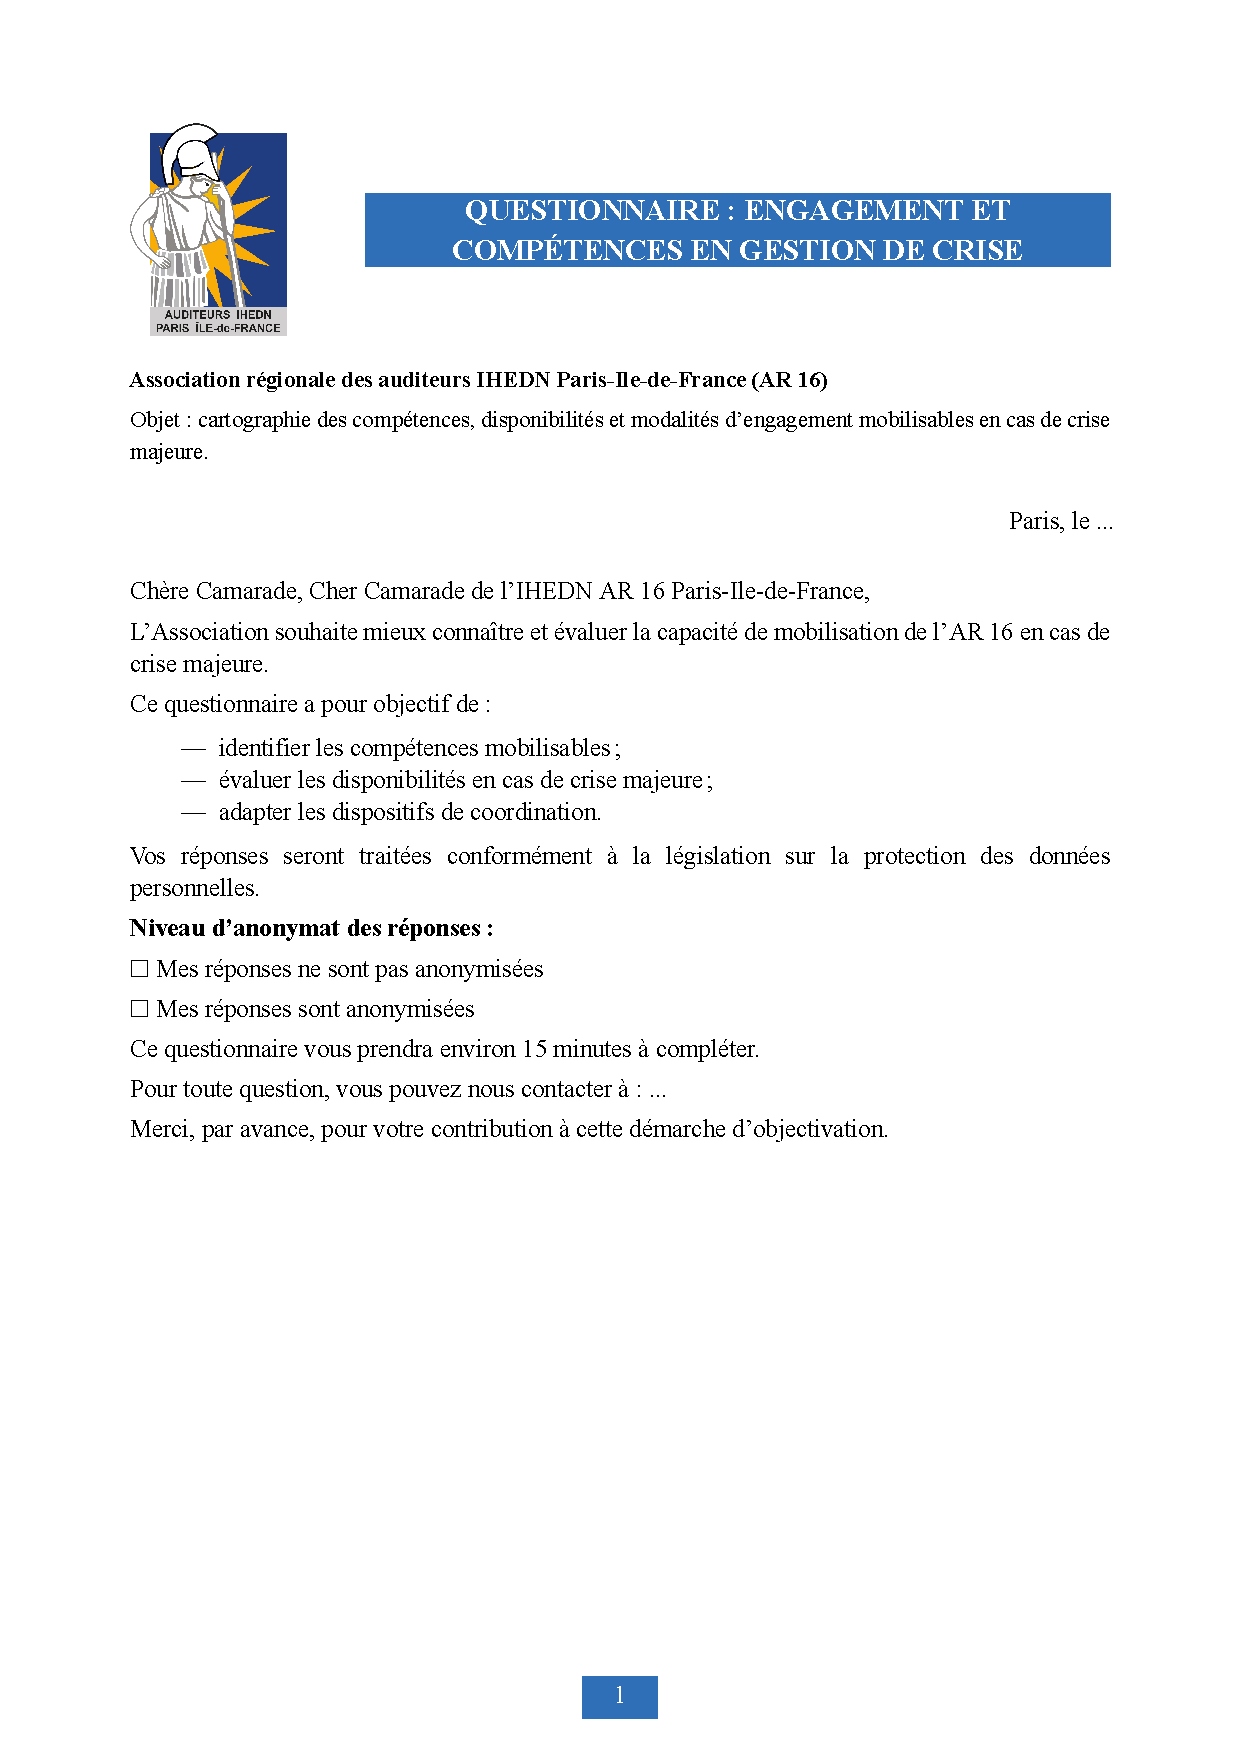
\includegraphics[page=1,width=0.95\textwidth]{QCM.pdf}
\end{tcolorbox}

\clearpage

\begin{tcolorbox}[
colback=gray!5,
colframe=black,
boxrule=0.5pt,
arc=3mm
]
\centering
\includegraphics[page=2,width=0.95\textwidth]{QCM.pdf}
\end{tcolorbox}

\clearpage

\printglossary[type=\acronymtype,title={Liste des acronymes}]

\clearpage

%\printbibliography[heading=bibintoc,title={Références bibliographiques}]

\addcontentsline{toc}{section}{Références bibliographiques}
\printbibheading[title={Références bibliographiques}]

\addcontentsline{toc}{subsection}{Articles de recherche}
\printbibliography[	keyword=article_de_recherche,
					title={Articles de recherche},
					sorting=nyt,
					heading=subbibliography]

\addcontentsline{toc}{subsection}{Rapports institutionnels}
\printbibliography[	keyword=rapport_institutionnel,
					title={Rapports institutionnels},
					sorting=nyt,
					heading=subbibliography]

\clearpage

\addcontentsline{toc}{subsection}{Ressources en ligne}
\printbibliography[	keyword=article_online,
					title={Ressources en ligne},
					sorting=nyt,
					heading=subbibliography]


\addcontentsline{toc}{subsection}{Ouvrages}
\printbibliography[	keyword=livre,
					title={Ouvrages},
					sorting=nyt,
					heading=subbibliography]

\end{document}
